%************************************************
\chapter{Introduction}\label{ch:introduction}
%************************************************

\begin{flushright}{\slshape The story so far: In the beginning the Universe was created. This has made a lot of people very angry and been widely regarded as a bad move.} \\ \medskip
    ---  The Restaurant at the End of the Universe, Douglas Adams 
\end{flushright}

The popularity of robotics is growing everywhere. Not only in the academic world, where various research activities are now applied to robotics but also in the industrial world, where companies are providing new commercial solutions involving robots. Even the general public is now more used to a society where robots coexist and collaborate with humans. The first model of iRobot Roomba was introduced in 2002, and today some young adults grew up in a world where robots are part of the household.

The current evolution of robotics as a field is similar, in a way, to the growth in popularity of mobile phones, first, and smartphones, later.  Originally, the idea of a personal wireless communication system was only possible in science fiction, then scientific progress and new technologies made it possible. At first only for very few applications (\eg, the military, the railroad system), but later it grew exponentially, and today it is part of our everyday life. Many factors made this leap possible: first of all, technological advancements, such as miniaturisation, battery life extension, increase in display quality, cheaper computational power, additionally, a sense of need, people felt that a mobile phone was a great addition to their life, lastly, standardisation, accessible development environments, and multiple abstraction layers.

The same was for robots, initially no more than toys, mechanical puppets and mysterious automata. They existed, as truly autonomous agents, only in the minds and works of writers and directors, and even today we are not able to match those visions. As soon as technology made it possible, the first robotic arms were developed. Initially applied to heavy industry to replace human in dangerous and highly specialised tasks, later, technical refinements and functionality extensions made them suitable for healthcare and collaboration with humans. From here it was an explosion of different technologies, shapes and applications. Robotic arms evolved in precision, power and dexterity,  from the massive industrial arms to the agile surgical robots.  Soon after the development of the first sophisticated arms, many researchers tried to realise the vision of a full humanoid robot, but, even today, after much progress, we are not able to fully replicate the complexity of the human body. Mobile platforms were the next logical step: robots able to autonomously explore and navigate the environment, robots able to reason on what they detect and to react accordingly.

In the last two decades, robotics has been applied in numerous fields, and robots assumed a myriad of shapes and functionalities. In industry, robots are used for welding, painting, drilling, cutting, handling dangerous materials, moving heavy objects, pick-and-place, inventory management. In healthcare, today, surgical robots are the norm, but advancement in soft robotics made robots suitable for rehabilitation and elderly care. Most of the recent discoveries of planetary science exist thanks to rovers, autonomous mobile robots that can, unassisted, explore the surface of planets, asteroids and comets. Moreover, maintenance in outer space is hazardous for humans and often impossible, only robotic arms and autonomous probes can perform it. Back on Earth, in our houses and cities, robots are not an unusual sight. There are robotic vacuum cleaners and lawnmowers,  autonomous robots deliver packages directly to the front door, and self-driving public transportation is a reality in various cities. Fully autonomous cars are still only prototypes, however not because of technological limitations, but mostly for economic, social and legal reasons. Thanks to the recent progress in human-robot interaction, the sight of a robotic waiter or concierge, while marvellous, is not completely unexpected. Lastly, unmanned autonomous vehicles (\eg, off-road vehicles, drones, boats, submarines),  have been used successfully in search and rescue missions and to operate in dangerous environments, such as mountain peaks, volcanos, disaster zones, and contaminated areas.

\begin{figure}
    \centering
    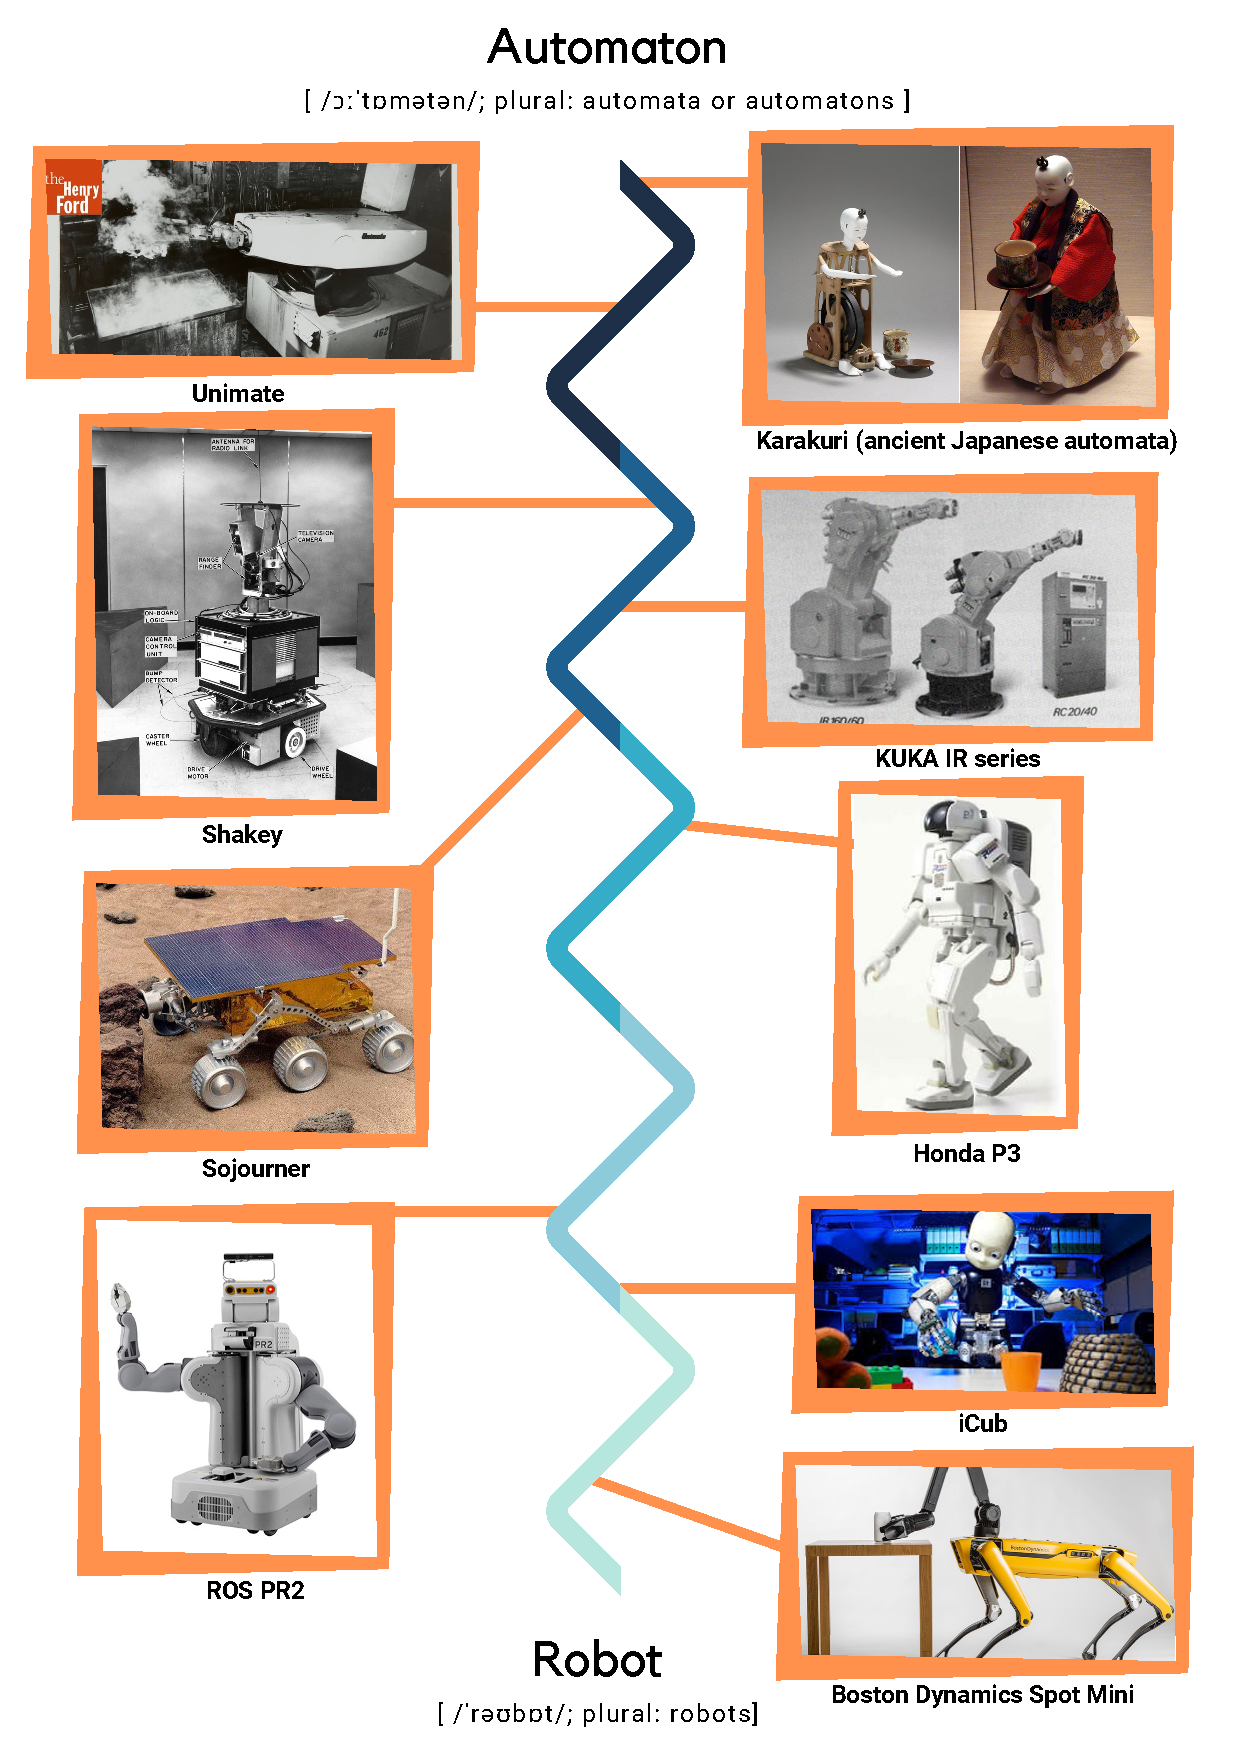
\includegraphics[width=\textwidth]{gfx/history}
    \caption{A brief history of robotics. From the ancient automata to modern robots.}\label{fig:history}
\end{figure}

In this brief history of robots, most of the progress and technological advancements seems related to the hardware: more responsive motors, more precise and reliable sensors, cheaper electronics and more computational power. All these advancements contributed to what is robotics today. However, the software has always been one of the main concerns of any roboticist. The implementation, the logic, is what makes the difference between a mechanism and an intelligent robot. Since their inception, robots have spawned a series of software solutions to implement their functionalities. For example, the Stanford Research Institute Problem Solver (STRIPS)~\cite{lifschitz1987semantics} is an automated planner developed for Shakey~\cite{nilsson1984shakey} that became the foundation of modern action languages. Modern robots have software architecture far more advanced than Shakey: they coordinate multiple sensors and actuators,  implement different functionalities, and often operate in real-time.

For these reasons, in the last twenty-five years, various efforts in robotic software revolved around the design of a solution to streamline and simplify the development process. The answer was the introduction of robotic middleware and frameworks and to rely on component-based designs. This approach fits perfectly the necessities of robotics, components encapsulate functionalities and promote reusability, while a pre-defined communication layer frees the developer from the burden of micromanaging the low-level interactions. After the first wave of ad hoc implementations, few frameworks rose in popularity and become standard de-facto for robot software development. Today, depending on the specific application, a developer can choose various frameworks or middleware: OROCOS~\cite{bruyninckx2002orocos} (or its derivation RoCK~\cite{joyeux2011robot}), for real-time application, SmartMDSD~\cite{dennis2016smartmdsd}, for a more complete and structured development environment, YARP~\cite{metta2006yarp}, for a more light-weight and data-centric approach, or ROS~\cite{quigley2009ros}, for more extensive support and development freedom.

Middleware and frameworks fuelled the progress of robotic systems, creating the current scenario of robot design and development. Hundreds of components are already available to anyone who wants to implement a robot and experts can set up the most common functionalities (\ie, teleoperation, mapping, indoor localisation and navigation) of a new system in a matter of days. However, the learning curve to reach this kind of expertise is quite steep and extending the functionalities of a robot beyond what is currently available requires a considerable effort not strictly related to the new functionality itself.

By recalling the parallel between robotics and smartphones, we are currently in robotics in the same situation developers were before the standardisation introduced by Android. Today, an Android developer can bootstrap and deploy a new application on millions of devices in few steps, thanks to abstraction layers that separate the development environment to the underlying hardware and operating system and thanks to advanced design, development and simulation tools. Of course, smartphones are not robots, and while there is a significant variability from one device to another (\eg, screen size, quality and number of cameras, sensors availability, type of mobile network, \etc), they cannot be compared to the incredible range of sensors, actuators, shapes and functionalities that exist in robotics. For this reason, while robotics can aim to achieve the same streamlined development of smartphones, the approach needs to be different.

\section{Motivations}
Middleware and frameworks created the present development landscape of robotics, but current approaches are not suitable any more for a constantly advancing robotic field. The personal experience of an all-around robotic expert still drives robotic software design and development. When developing a new system or application, it is expected that a developer has total expertise on the low-level functionalities provided by the underlying framework and the high-level functionalities to be implemented; while this was possible in the past, it is an unsustainable approach today. Not only it is necessary to create a distinction between different roles in the design and development process of a robot, but it is also necessary to provide them with the right tools to fulfil their tasks.

The \textit{system designer} needs tools to outline the architecture of the system and describe the high-level interactions and requirements of components. This can be achieved using a modelling language to describe components and their inner workings in an agnostic way with respect to the underlying framework. This approach, not only provides the right environment for the designer, but it also provides early detection of errors, an architectural overview of the system and system-level reusability. 

The \textit{component developer} should focus only on the implementation of the internal logic and not on the structure of the component itself, since this is the role of the designer. To do so, the component developer needs an environment that abstracts from the framework-related boilerplate code and provides a contained development space. Potentially, the logic implemented should be portable from one component to another, even if they are not based on the same framework, given they share the same design principles. Building on top of the modelling language used by the system designer, it is possible to achieve the ideal development environment by delegating to an automatic code generator most of the boilerplate implementation, and by defining a bounded reference component that can be used by the \textit{component developer} as a starting point.

The \textit{application developer} implements high-level functionalities, that should be independent of the underlying architecture of the robot. In practice, this means it should exist an abstraction layer between the low-level capabilities provided by one or more components and the high-level applications. There are a plethora of robots, with different configurations and implementations; however, it is possible to abstract most of the capabilities independently from the system. An example could be teleoperation: by defining linear and angular velocity of the mobile platform, it is possible to control any robot, independently from their physical configuration. The application developer should be able to implement high-level functionalities for multiple robots with minimal modifications by using these general interfaces. To achieve this, it is necessary to define the concept of capabilities, to identify them in a robot architecture and to provide a framework-independent way to interact with them.

\section{Thesis contributions}
Our proposed approach revolves around two key factors: formalise the design and development of robotic software and streamline the implementation process for the different experts involved. We developed methodologies, techniques and tools, each one focused on a different aspect or phase of the design and development process to assist each role on their specific task, but all interconnected to benefit one from another.

For the \textit{system designer} we exploited an existing modelling language to create a suitable description for robotic architectures. We relayed on the fact that the most popular middleware and frameworks adopt a \textit{component-connector} paradigm to create a generalised approach. Since the aim is to cover the entire development process by supporting all the actor involved, we then focused on creating a more specialised description to model ROS-based architectures. The generalised approach already covers the concept of components (\ie, nodes), ports (\ie, publishers, subscribers, service clients and servers) and connections (\ie, topics and services). At the same time, the specialised description goes more in details by providing models for messages and the internal structure and functionalities of the nodes.

The advantages for the \textit{system designer} are multiple; a model of the complete system gives an architectural overview which is otherwise impossible to achieve before runtime, moreover it is possible to check, before execution, the compatibility of the communication channels, a functionality that is usually unavailable in those frameworks and middleware that connect the component at start-up time. Additionally, the designer can rely on a library of already existing templates, and this makes the design of the system more manageable and the resulting architecture more robust. Lastly, by basing this work on an existing modelling language, we allow the designer to exploit all the other tools available for the language, such as latency estimation, computational load, hardware allocation and fault propagation.

The \textit{component developer} often works together with the \textit{domain expert}. With our work, we provide support for both roles and their interaction. From the model created by the \textit{system designer} we provide an automatic code generation to ROS. The target implementation is based on a reference node specifically engineered to minimise the amount of boilerplate code and to provide additional features that are usually managed by the \textit{component developer}, few examples are internal life cycle of the node, well-defined initialisation procedure, encapsulation of parameters and internal state, clear separation between the middleware and implementation. The latter is particularly important for the role of the \textit{domain expert}; their contribution to the functionalities of a robot is fundamental, they provide control software, local and global planning algorithms, robot behaviours, and more. Since they are expert of a specific domain and carrier of specialised and valuable knowledge, they often do not, and ideally, should not implement the component directly, they should have access to a suitable interface. In our proposed model and automatic code generation approach a \textit{domain expert} can implement a functionality independently and then embed it in the model, the automatic code generator will include it in the final implementation.

Lastly, for the \textit{application developer}, we developed the concept of robot capabilities. We define them as low or medium-level functionalities (\eg, directional movement or navigation) and a developer can use them to interact with the robot (\ie, to send commands of varying complexity) and to receive information from the robot (\ie, to read sensor measurements). The capabilities are defined manually by analysing the configuration and functionalities of different types of robots (\ie, mobile platforms, drones and manipulators), but the active capabilities on a running system are extracted automatically by analysing the ROS graph.

On top of the concept of capabilities, we developed an abstraction layer to decouple the application from the underlying middleware or framework. In our approach, we implemented a bridge between the capabilities and, consistently, ROS-based systems. To do so, we developed a dynamic node that can manage bidirectional communication with an external system through different communication channels. We provide dynamically defined APIs a developer can use to interact with the robot through capabilities. To test the effectiveness of this approach in simplifying robot development, we designed a web interface that can be used to create visual algorithms to program a remote robot.

Even if it is not evident at first glance, all these methodologies, techniques and tools are all part of a continuous design and development process. The \textit{system designer} uses the modelling tools and templates to define the architecture of the system. He can embed directly the reference to the source code developed by the \textit{domain expert}, and, using properties, even enrich the component with their evoked capability. Through automatic code generation most of the source code is already available with minimal effort, at this point the \textit{component developer} can finalise the implementation by adding anything that cannot be automatically generated, for example, special interfaces with the hardware components or specific initialisation and shutdown procedures. The result is a robust system where all the components are known, well designed and well implemented, and this is the suitable starting point for an \textit{application developer} to exploit safely the abstraction layer defined using robot capabilities.

\section{Thesis outline}
This thesis is divided into eight chapters:
\begin{itemize}
\item Chapter~\ref{ch:Related} gives an overview of technologies, techniques, methodologies and approaches related to the work presented in this thesis.  We focus mostly on software engineering and model-driven approaches, and how they are used in general and robotics applications.
\item Chapter~\ref{ch:Background} provides details of the two main technologies used in this thesis: the Robot Operating System (ROS) and the Architecture Analysis \& Design Language (AADL).
\item Chapter~\ref{ch:Modelling} presents our model-based approach. First, we introduce a high-level description of a generic component-based robotic architecture, and then we show how AADL can be used to model it. The chapter continues by extending the approach to ROS; initially by describing a single node, and then by designing a complete architecture. We conclude by finalising the model definition using two different and interchangeable data modelling languages.
\item Chapter~\ref{ch:code-gen} presents our code generation toolchain. First, we describe the target of the code generation process, in particular, how we engineered an enhanced ROS node with additional functionalities, and how it can be used to implement custom ROS nodes. All the phases of the two-step code generation process are described next. The chapter closes with a complete example from the AADL model to the ROS/C++ implementation.
\item Chapter~\ref{ch:capabilities} presents our ontology-based robot abstraction. The chapter opens by describing the ontology used to define ROS, the binding between ROS elements and the capabilities, and the capabilities taxonomy. The abstraction is used to define robot APIs that can be used to exploit specific capabilities. We conclude by analysing how the ontology-based abstraction benefits the model-based approach and vice versa.
\item Chapter~\ref{ch:Experiment} focuses on the experimental evaluation of our work. We present two scenarios. One uses the architecture of an autonomous wheelchair to demonstrate the functionalities of our model-based development approach. The other exploit our ontology-based abstraction to create a set of web APIs that developer with no experience in robotics can use to program different robotic platforms.
\item Chapter~\ref{ch:Conclusions} draws relevant conclusions of this work and present potential extensions and future works.
\end{itemize}

\newpage

\section{Publications}
\begin{itemize}
\item \textbf{G. Bardaro}, M. Matteucci \\
Using AADL to model and develop ROS-based robotic application~\cite{bardaro2017using} \\
\textit{International Conference on Robotic Computing (IRC)}, 2017
\item \textbf{G. Bardaro}, A. Semprebon, M. Matteucci \\
AADL for robotics: a general approach for system architecture modeling and code generation~\cite{bardaro2017aadl} \\
\textit{Journal of Software Engineering for Robotics (JOSER)}, 2017
\item I. Tiddi, E. Bastianelli, \textbf{G. Bardaro}, M. d'Aquin, E. Motta \\
An ontology-based approach to improve the accessibility of ROS-based robotic systems~\cite{tiddi2017ontology} \\
\textit{Knowledge Capture Conference (KCap)}, 2018 \\
\item I. Tiddi, E. Bastianelli, \textbf{G. Bardaro}, E Motta \\
A User-friendly Interface to Control ROS Robotic Platforms~\cite{tiddi2018user} \\
\textit{International Semantic Web Conference (ISWC)}, 2018
\item \textbf{G. Bardaro}, A. Semprebon, M. Matteucci \\
A use case in model-based robot development using AADL and ROS~\cite{bardaro2018use} \\
\textit{International Workshop on Robotics Software Engineering (RoSE)}, 2018
\item \textbf{G. Bardaro}, A. Semprebon, A. Chiatti, M. Matteucci \\
From Models to Software Through Automatic Transformations: An AADL to ROS End-to-End Toolchain~\cite{bardaro2019models} \\
\textit{International Conference on Robotic Computing (IRC)}, 2019
\end{itemize}

%*****************************************
